\documentclass[a4paper,12pt,twoside]{article}
\usepackage[left=1in,right=1in,top=1in,bottom=1in]{geometry}

\usepackage{xeCJK}
\setCJKmainfont{Songti TC}
\setCJKfamilyfont{kai}{Songti TC}
\newcommand{\kai}{\CJKfamily{kai}} % 用 \kai{使用楷書}

\usepackage{lmodern}
\usepackage{titling}
\usepackage{titlesec}
\usepackage{graphicx}
\usepackage{float}
\usepackage{amsmath, amsthm, amssymb, amsfonts, mathrsfs}
\usepackage{upgreek} % 直立的希臘字母

\usepackage[shortlabels]{enumitem}
\usepackage{setspace}
\renewcommand{\baselinestretch}{1.5}
\usepackage[colorlinks]{hyperref}
\usepackage{fancyvrb}
\usepackage{fancyhdr}
\usepackage{multicol}
\usepackage{caption}
\usepackage{listings}
\usepackage{bm}
\usepackage{bbm} % for \mathbbm{1} (indicator function)
\usepackage{centernot}
\usepackage{mdframed}
\usepackage{tikz}
\usetikzlibrary{patterns, arrows.meta, positioning}
\usepackage[nameinlink, capitalise]{cleveref}
\usepackage{diagbox}
\usepackage{booktabs}
\usepackage{multirow,array}
\usepackage{tabularx}
\usepackage{mathtools}
\usepackage{indentfirst} % 首段 indent
\setlength{\parindent}{2em}
\usepackage{cancel} % 數學式子畫線槓掉
\newcommand\mcancel[2][red]{\setbox0=\hbox{$#2$}%
\rlap{\raisebox{.45\ht0}{\textcolor{#1}{\rule{\wd0}{1pt}}}}#2}
\usepackage{datetime2}

\AtBeginDocument{%
 \setlength{\abovedisplayskip}{6pt}
 \setlength{\belowdisplayskip}{6pt}
 \setlength{\abovedisplayshortskip}{4pt}
 \setlength{\belowdisplayshortskip}{4pt}
}

\definecolor{codegreen}{rgb}{0,0.6,0}
\definecolor{codegray}{rgb}{0.5,0.5,0.5}
\definecolor{codepurple}{rgb}{0.58,0,0.82}
\definecolor{backcolour}{rgb}{0.95,0.95,0.92}

\lstdefinestyle{mystyle}{
 backgroundcolor=\color{backcolour},
 commentstyle=\color{codegreen},
 keywordstyle=\color{magenta},
 numberstyle=\tiny\color{codegray},
 stringstyle=\color{codepurple},
 basicstyle=\ttfamily\footnotesize,
 breakatwhitespace=false,
 breaklines=true,
 captionpos=b,
 keepspaces=true,
 numbers=left,
 numbersep=5pt,
 showspaces=false,
 showstringspaces=false,
 showtabs=false,
 tabsize=2
}
\lstset{style=mystyle}

\hypersetup{citecolor=blue, linkcolor=blue, urlcolor=blue}

\DeclareMathOperator{\supp}{supp}
\DeclareMathOperator{\skewness}{Skewness}
\DeclareMathOperator{\DU}{D-U}
\DeclareMathOperator{\CU}{C-U}
\DeclareMathOperator{\Geo}{Geo}
\DeclareMathOperator{\Pois}{Pois}
\DeclareMathOperator{\Gam}{Gam}
\DeclareMathOperator{\LN}{LogN}
\DeclareMathOperator{\cov}{Cov}
\DeclareMathOperator*{\argmax}{arg\,max}
\DeclareMathOperator*{\argmin}{arg\,min}
\DeclareMathOperator{\re}{Re}
\DeclareMathOperator{\im}{Im}

\newcommand{\N}{\mathbb{N}}
\newcommand{\Z}{\mathbb{Z}}
\newcommand{\Q}{\mathbb{Q}}
\newcommand{\R}{\mathbb{R}}
\newcommand{\C}{\mathbb{C}}
\newcommand{\G}{\mathcal{G}}
\newcommand{\mP}{\mathbb{P}}
\newcommand{\F}{\mathcal{F}}
\newcommand{\B}{\mathcal{B}}
\newcommand{\1}{\mathbbm{1}}
\newcommand{\Poi}{\text{Poi}}
\newcommand{\Var}{\text{Var}}
\newcommand{\as}{\text{a.s.}}
\newcommand{\vect}[1]{\boldsymbol{\mathbf{#1}}}
\newcommand{\paren}[1]{\left({#1}\right)}
\newcommand{\brk}[1]{\left[{#1}\right]}
\newcommand{\curl}[1]{\left\{{#1}\right\}}
\renewcommand{\lambda}{\lambdaup}

\theoremstyle{definition} % 定理環境 style 改用正體
\newtheorem{theorem}{定理}
\newtheorem{definition}{定義}
\newtheorem*{definition*}{定義}
\newtheorem{example}{例子}
\newtheorem{exercise}{練習}
\newtheorem{corollary}{推論}
\newtheorem{property}{性質}
\newtheorem{prop}{命題}
\newtheorem{lemma}{引理}
\newtheorem{problem}{問題}
\newtheorem*{remark}{註}

\renewcommand{\figurename}{圖}
\renewcommand{\tablename}{表}

\DeclareMathOperator{\var}{Var}
\DeclareMathOperator{\corr}{corr}
\DeclareMathOperator{\rank}{rank}
\DeclareMathOperator{\MSE}{MSE}
\DeclareMathOperator{\SSE}{SSE}
\DeclareMathOperator{\SST}{SST}
\DeclareMathOperator{\SSR}{SSR}
\DeclareMathOperator{\sgn}{sign}
\DeclareMathOperator{\alt}{Alt}
\DeclareMathOperator{\adj}{adj}
\DeclareMathOperator{\curlOp}{curl}
\DeclareMathOperator{\spn}{span}
\DeclareMathOperator{\sse}{SSE}
\DeclareMathOperator{\tr}{tr}

\newcommand{\ep}{\varepsilon}
\newcommand{\p}{\partial}
\newcommand{\abs}[1]{\left|#1\right|}
\newcommand\norm[1]{\left\lVert#1\right\rVert}
\newcommand{\innerprod}[1]{\langle#1\rangle}
\newcommand{\ds}{\displaystyle}
\newcommand{\blank}{\rule[-1mm]{1.5cm}{0.1mm}}
\newcommand{\dint}{\displaystyle\int}
\renewcommand{\bar}{\overline}

\newtheoremstyle{remark}{}{}{}{}{\bfseries\sffamily}{.}{.5em}{#1}
\theoremstyle{remark}

\newtheorem*{remark*}{\textit{Remark}}
\newtheorem*{solution*}{解}

\AtEndEnvironment{solution*}{\hfill$\square$}
\newtheorem*{hint*}{Hint}


\usepackage{tcolorbox}
\tcbuselibrary{skins,breakable}
\usetikzlibrary{patterns,decorations.pathreplacing,decorations.markings,decorations.shapes,decorations.pathmorphing,calc}

\newenvironment{example-non}[1][]{\vspace{0.8em}\noindent\textbf{#1}\quad}{\vspace{0.8em}}
\newenvironment{solution}{\par\noindent\textbf{解}\quad}{\par\vspace{0.8em}}

\fancypagestyle{firstpage}{
  \fancyhf{}
  \fancyhead[R]{\small《高中數學實驗教材》第 4 冊（自然組）}
  \fancyhead[L]{\small 附錄二\quad 圓系}
  \fancyfoot[C]{\thepage}
}

\pagestyle{fancy}
\setlength{\headheight}{14pt}
\renewcommand{\headrulewidth}{0.5pt}
\renewcommand{\footrulewidth}{0pt}
\fancyhead{}
\fancyhead[LE]{\small 《高中數學實驗教材》第四冊（自然組）}
\fancyhead[RO]{\small 附錄二\quad 圓系}
\fancyfoot[C]{\thepage}

\title{\LARGE\textbf{《高中數學實驗教材》第四冊（自然組）}\\[0.5em] \Large\textbf{附錄二\quad 圓系}}
\author{\textbf{高中數學實驗教材編輯小組}\quad 編著}
\date{民國六十五年（1976）三版}

\begin{document}

\maketitle
\thispagestyle{firstpage}

\tableofcontents
\newpage

% =========================================================================
% 《高中數學實驗教材》第四冊（自然組）
% 附錄二 圓系
% =========================================================================

\section*{附錄二\quad 圓系}
\addcontentsline{toc}{section}{附錄二\quad 圓系}
\label{sec:b4-a2}

在第三冊第四章我們講過直線系．例如利用兩個參數 $\alpha$ 與 $\beta$，定理 4 說：通過二相交的直線
\begin{align}
L_1:&\; a_1 x + b_1 y + c_1 = 0 \label{eq:b4-a2-1} \\
L_2:&\; a_2 x + b_2 y + c_2 = 0 \label{eq:b4-a2-2}
\end{align}
的交點的直線方程式可表為
\begin{equation}
L:\; \alpha(a_1 x + b_1 y + c_1) + \beta(a_2 x + b_2 y + c_2) = 0, \label{eq:b4-a2-3}
\end{equation}
即當 $\alpha$ 與 $\beta$ 變動時，我們可得一系列的直線．

我們知道只要 $L$ 不正好代表 $L_2$，則 $\alpha \neq 0$，此時將 \eqref{eq:b4-a2-3} 式兩端遍除 $\alpha$，並設 $k = \frac{\beta}{\alpha}$，\eqref{eq:b4-a2-3} 式可改寫為（定理 5）
\[
L:\; (a_1 x + b_1 y + c_1) + k(a_2 x + b_2 y + c_2) = 0.
\]
這樣的形式比 \eqref{eq:b4-a2-3} 式在計算時有用，因只牽涉到一個參數 $k$，只要再加一個條件就能決定 $L$ 的確實位置及其方程表示．

現在我們要來看圓的方程式中含有可變動的參數時，隨著該參數值的變動而得到一系列的圓．

事實上在介紹自由度的觀點時，我們已將空間中的點可能伸展的運動範圍的觀點應用到一般集合的元素上，其中〔例 19〕中的集合 $S_1$，就是平面上所有以原點為中心的同心圓的集合，我們可以經由指定它們的半徑長 $k$，來準確地挑出這集合中的一圓．$k$ 是我們所選的參數，此一集合稱為同心圓系，仍記作 $S_1$，
\[
S_1 = \{C_k \mid C_k: x^2+y^2=k^2, \; k \in \mathbf{R}\}
\]
其中 $C_k: x^2+y^2=k^2$ 稱為圓系 $S_1$ 的參數方程式．

同樣的
\[
\{C_k \mid C_k: (x-k)^2+y^2=1, \; k \in \mathbf{R}\}
\]
為所有半徑為 1，圓心在 $X$ 軸的圓系．

\begin{center}
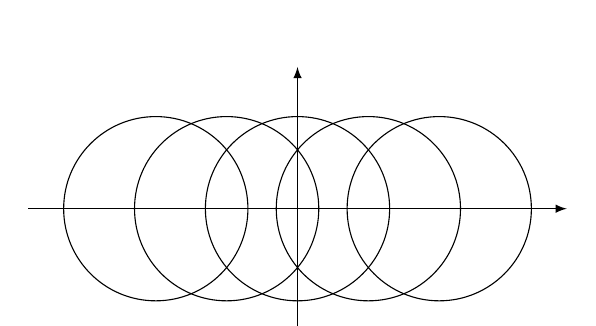
\begin{tikzpicture}[>=latex, scale=0.9]
  \draw[->] (-3.8,0) -- (3.8,0);
  \draw[->] (0,-1.8) -- (0,2.0);
  \foreach \k in {-2.0, -1.0, 0, 1.0, 2.0} {
    \draw (\k, 0) circle (1.3);
  }
\end{tikzpicture}
\end{center}

又
\[
\{C_k \mid C_k: x^2+y^2+2kx-a^2=0, \; k \in \mathbf{R}\}
\]
為所有通過 $(0, a)$ 和 $(0, -a)$ 的圓系．

\begin{center}
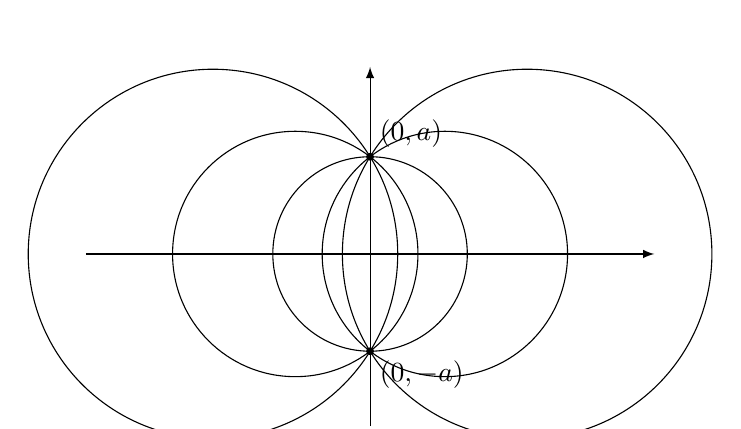
\begin{tikzpicture}[>=latex, scale=0.95]
  \draw[->] (-3.8,0) -- (3.8,0);
  \draw[->] (0,-2.3) -- (0,2.5);
  
  \coordinate (P1) at (0, 1.3);
  \coordinate (P2) at (0, -1.3);
  \fill (P1) circle (1.5pt) node[above right] {$(0, a)$};
  \fill (P2) circle (1.5pt) node[below right] {$(0, -a)$};
  
  % 5 Circles through (0, 1.3) and (0, -1.3)
  \draw (0, 0) circle (1.3);
  \draw (1.0, 0) circle ({sqrt(1.0*1.0 + 1.3*1.3)});
  \draw (-1.0, 0) circle ({sqrt(1.0*1.0 + 1.3*1.3)});
  \draw (2.1, 0) circle ({sqrt(2.1*2.1 + 1.3*1.3)});
  \draw (-2.1, 0) circle ({sqrt(2.1*2.1 + 1.3*1.3)});
\end{tikzpicture}
\end{center}

而我們在 § III-6 講圓的正交與鏡射時也做出一個通過定點 $P(a, b)$ 且與定圓 $C_0$ 正交的圓系，此圓系中每一圓皆過另一點 $P'$，即點 $P$ 對於圓 $C_0$ 的鏡射點，其圓心在線段 $\overline{PP'}$ 的垂直平分線上，若定圓 $C_0$ 的方程式為
\[
C_0: x^2+y^2=r^2
\]
則圓系的參數方程式為
\[
C: x^2+y^2+2Dx+2Ey+r^2=0
\]
其中 $D$ 與 $E$ 滿足關係
\[
2Da+2Eb = -(a^2+b^2+r^2).
\]

\subsection*{§ 1\quad 共軸圓系}
\addcontentsline{toc}{subsection}{§ 1\quad 共軸圓系}

在各種圓系中以共軸圓系較常用到．

給了兩個圓心相異的定圓
\begin{align*}
C:&\; x^2+y^2+2Dx+2Ey+F=0 \\
C':&\; x^2+y^2+2D'x+2E'y+F'=0
\end{align*}
考慮由方程式
\[
C_t: (x^2+y^2+2Dx+2Ey+F) + t(x^2+y^2+2D'x+2E'y+F') = 0
\]
所表示的圓系，我們以下要利用等切軸來說明此圓系具有共同的等切軸而稱其為由 $C$ 與 $C'$ 產生的共軸圓系．

\begin{prop}[命題 1]
平面上所有到兩（圓心相異的）圓
\begin{align*}
C:&\; x^2+y^2+2Dx+2Ey+F=0 \\
C':&\; x^2+y^2+2D'x+2E'y+F'=0
\end{align*}
有等長切線的點的軌跡為一直線
\[
L:\; 2(D-D')x + 2(E-E')y + F-F' = 0
\]
此直線稱為 $C$ 與 $C'$ 的\textbf{等切軸}．
\end{prop}

\begin{center}
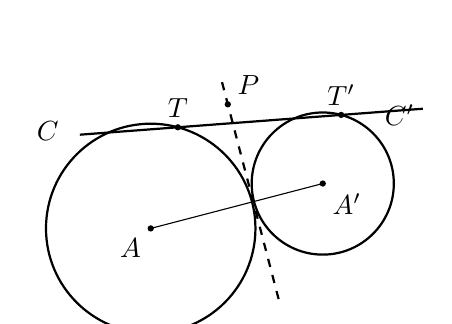
\begin{tikzpicture}[>=latex, scale=0.95]
  % Top: externally tangent circles
  \coordinate (A) at (-1.2, -0.25);
  \coordinate (Ap) at (1.1, 0.35);
  
  \draw[thick] (A) circle (1.4);
  \draw[thick] (Ap) circle (0.95);
  
  \draw (A) -- (Ap);
  \fill (A) circle (1.2pt) node[below left] {$A$};
  \fill (Ap) circle (1.2pt) node[below right] {$A'$};
  
  \node[above left] at (-2.3, 0.8) {$C$};
  \node[above right] at (1.8, 1.0) {$C'$};
  
  % Tangency point on line of centers
  \coordinate (Touch) at ($(A)!1.4/(1.4+0.95)!(Ap)$);
  
  % Radical axis (perpendicular to line of centers at Touch)
  \draw[dashed, thick] ($(Touch)!-1.4!90:(Ap)$) -- ($(Touch)!1.8!90:(Ap)$);
  
  % Point P on radical axis
  \coordinate (P) at ($(Touch)!1.4!90:(Ap)$);
  \fill (P) circle (1.2pt) node[above right] {$P$};
  
  % Common external tangent through P, touching C at T and C' at T'
  \coordinate (T) at ($(A)+(75:1.4)$);
  \coordinate (Tp) at ($(Ap)+(75:0.95)$);
  \draw[thick] ($(T)!-0.6!(Tp)$) -- ($(Tp)!-0.5!(T)$);
  
  \fill (T) circle (1.2pt) node[above] {$T$};
  \fill (Tp) circle (1.2pt) node[above] {$T'$};
\end{tikzpicture}
\\[1.5em]
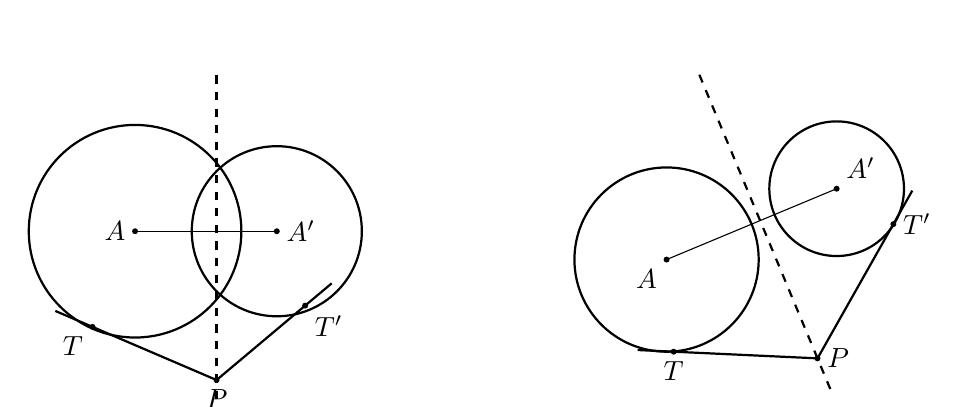
\begin{tikzpicture}[>=latex, scale=0.9]
  % Intersecting circles (bottom-left)
  \begin{scope}[shift={(-4.2,0)}]
    \coordinate (A) at (-1.1, 0);
    \coordinate (Ap) at (0.9, 0);
    
    \draw[thick] (A) circle (1.5);
    \draw[thick] (Ap) circle (1.2);
    \draw (A) -- (Ap);
    
    \fill (A) circle (1.2pt) node[left] {$A$};
    \fill (Ap) circle (1.2pt) node[right] {$A'$};
    
    % Radical axis (common chord extended)
    \draw[dashed, thick] (0.05, 2.2) -- (0.05, -2.4);
    
    \coordinate (P) at (0.05, -2.1);
    \fill (P) circle (1.2pt) node[below] {$P$};
    
    % Tangents from P
    \coordinate (T) at (-1.7, -1.35);
    \coordinate (Tp) at (1.3, -1.05);
    \draw[thick] (P) -- ($(P)!1.3!(T)$);
    \draw[thick] (P) -- ($(P)!1.3!(Tp)$);
    
    \fill (T) circle (1.2pt) node[below left] {$T$};
    \fill (Tp) circle (1.2pt) node[below right] {$T'$};
  \end{scope}
  
  % Non-intersecting circles (bottom-right)
  \begin{scope}[shift={(3.5,0)}]
    \coordinate (A) at (-1.3, -0.4);
    \coordinate (Ap) at (1.1, 0.6);
    
    \draw[thick] (A) circle (1.3);
    \draw[thick] (Ap) circle (0.95);
    \draw (A) -- (Ap);
    
    \fill (A) circle (1.2pt) node[below left] {$A$};
    \fill (Ap) circle (1.2pt) node[above right] {$A'$};
    
    % Radical axis (perpendicular to AA')
    \coordinate (Mid) at ($(A)!0.55!(Ap)$);
    \draw[dashed, thick] ($(Mid)!-2.2!90:(Ap)$) -- ($(Mid)!2.0!90:(Ap)$);
    
    \coordinate (P) at ($(Mid)!-1.8!90:(Ap)$);
    \fill (P) circle (1.2pt) node[right] {$P$};
    
    % Tangents from P
    \coordinate (T) at (-1.2, -1.7);
    \coordinate (Tp) at (1.9, 0.1);
    \draw[thick] (P) -- ($(P)!1.25!(T)$);
    \draw[thick] (P) -- ($(P)!1.25!(Tp)$);
    
    \fill (T) circle (1.2pt) node[below] {$T$};
    \fill (Tp) circle (1.2pt) node[right] {$T'$};
  \end{scope}
\end{tikzpicture}
\end{center}

\begin{proof}
設點 $P(X, Y)$ 到 $C$ 與 $C'$ 的切線等長，設切點各為 $T$ 與 $T'$，則（作業 35，第三章）知
\begin{align*}
|\overline{PT}|^2 &= X^2+Y^2+2DX+2EY+F \\
&= X^2+Y^2+2D'X+2E'Y+F' = |\overline{PT'}|^2
\end{align*}
即 $P$ 點的座標滿足下方程式
\[
2(D-D')X + 2(E-E')Y + (F-F') = 0
\]
故其軌跡為一直線．

（注意此方程式是 $C$ 與 $C'$ 兩個方程式的「差」）
\end{proof}

\subsubsection*{作業 1}
試證兩圓的等切軸與其連心線互相垂直．

（提示：比較等切軸的法向量及連心線向量）

\begin{prop}[命題 2]
給定兩圓 $C$ 與 $C'$ 如命題 1，則圓系
\[
\{C_t \mid C_t(x^2+y^2+2Dx+2Ey+F) + t(x^2+y^2+2D'x+2E'y+F') = 0\}
\]
中任意二圓的等切軸均為 $C$ 與 $C'$ 的等切軸．

（因為圓系中圓共有一等切軸，故稱其為由 $C_1$ 與 $C_2$ 所產生的共軸圓系）
\end{prop}

\begin{proof}
設 $C_{t_1}$ 與 $C_{t_2}$ 為圓系中二圓：
\begin{align*}
C_{t_1}:&\; (x^2+y^2+2Dx+2Ey+F) + t_1(x^2+y^2+2D'x+2E'y+F') = 0 \\
C_{t_2}:&\; (x^2+y^2+2Dx+2Ey+F) + t_2(x^2+y^2+2D'x+2E'y+F') = 0
\end{align*}
化成標準式得：
\begin{align*}
C_{t_1}:&\; x^2+y^2+2\left(\frac{D+t_1 D'}{1+t_1}\right)x + 2\left(\frac{E+t_1 E'}{1+t_1}\right)y + \frac{F+t_1 F'}{1+t_1} = 0 \\
C_{t_2}:&\; x^2+y^2+2\left(\frac{D+t_2 D'}{1+t_2}\right)x + 2\left(\frac{E+t_2 E'}{1+t_2}\right)y + \frac{F+t_2 F'}{1+t_2} = 0
\end{align*}
故其等切軸方程式為：
\[
2\left(\frac{D+t_1 D'}{1+t_1} - \frac{D+t_2 D'}{1+t_2}\right)x + 2\left(\frac{E+t_1 E'}{1+t_1} - \frac{E+t_2 E'}{1+t_2}\right)y + \left(\frac{F+t_1 F'}{1+t_1} - \frac{F+t_2 F'}{1+t_2}\right) = 0
\]
整理化簡後即成：
\[
\frac{t_2-t_1}{(1+t_1)(1+t_2)} [2(D-D')x + 2(E-E')y + (F-F')] = 0
\]
此即為 $C$ 與 $C'$ 的等切軸方程式．
\end{proof}

容易看出：若圓 $C$ 與 $C'$ 相交於兩點，則其等切軸即為其公共弦，事實上我們有：

\begin{prop}[命題 3]
若 $C$ 與 $C'$ 相交，則由 $C$ 與 $C'$ 所產生的共軸圓系即為由所有過此二交點的圓所組成的圓系．
\end{prop}

\begin{proof}
設 $C$ 與 $C'$ 的交點為 $B_1(x_1, y_1)$ 和 $B_2(x_2, y_2)$，則
\[
\text{因 } B_1 \in C \cap C' \implies
\begin{cases}
x_1^2+y_1^2+2Dx_1+2Ey_1+F = 0 \\
x_1^2+y_1^2+2D'x_1+2E'y_1+F' = 0
\end{cases}
\]
所以
\[
(x_1^2+y_1^2+2Dx_1+2Ey_1+F) + t(x_1^2+y_1^2+2D'x_1+2E'y_1+F') = 0
\]
對任意實數 $t$ 皆成立．此即表示 $B_1 \in C_t$．

同理可證 $B_2 \in C_t$ 對任意 $t$ 成立，故知 $C_t$ 均過 $B_1$ 與 $B_2$．

反之 $\bar{C}$ 設為任意過 $B_1$ 與 $B_2$ 的圓．若 $\bar{C}$ 為 $C'$，則由定義知 $\bar{C}$ 屬於 $C$ 與 $C'$ 所產生的圓系．若 $\bar{C} \neq C'$，在 $\bar{C}$ 上取一點 $Q(X, Y)$，$Q$ 不在 $C'$ 上，則
\[
X^2+Y^2+2D'X+2E'Y+F' \neq 0\footnote{原書印為 $X^2+Y^2+2D'Z+2E'Y+F \ne 0$，其中 $Z$ 誤植，常數項脫落撇號，校訂為 $2D'X$ 及 $F'$．}．
\]
若取
\[
t = -\frac{X^2+Y^2+2DX+2EY+F}{X^2+Y^2+2D'X+2E'Y+F'}
\]
則容易看出 $C_t$ 過 $B_1$ 與 $B_2$ 及 $Q$ 點，因三點決定一圓，故知 $C_t = \bar{C}$ 即 $\bar{C}$ 為共軸圓系中的一圓．
\end{proof}

\subsubsection*{作業 2}
\begin{itemize}[leftmargin=2em]
  \item[(i)] 試證二相交圓的等切軸即為其公共弦．
  \item[(ii)] 試證二相切圓的等切軸即為其公切線．
\end{itemize}

\begin{prop}[命題 $3'$]
若 $C$ 與 $C'$ 相切，則由 $C$ 與 $C'$ 所產生的共軸圓系即為由所有與其公切線切於公切點的圓所組成的圓系．
\end{prop}

\begin{proof}
設 $C$ 與 $C'$ 切於點 $B(x_0, y_0)$，則 $C$ 與 $C'$ 在點 $B$ 的切線重合，易證 $B$ 點在 $C_t$ 上，而 $C_t$ 在 $B$ 點的切線方程式為：
\begin{align*}
0 &= x_0 x + y_0 y + \left(\frac{D+tD'}{1+t}\right)(x+x_0) + \left(\frac{E+tE'}{1+t}\right)(y+y_0) + \left(\frac{F+tF'}{1+t}\right) \\
&= \frac{1}{1+t} [(x_0 x + y_0 y + D(x+x_0) + E(y+y_0) + F) + t(x_0 x + y_0 y + D'(x+x_0) + E'(y+y_0) + F')]
\end{align*}
故知為同一直線，即為 $C$ 與 $C'$ 的等切軸．

反之，設圓 $\bar{C}$ 切 $C$ 與 $C'$ 的公切線 $L$ 於點 $B$．若 $\bar{C}$ 為 $C'$，則不必再證，若 $\bar{C} \neq C'$ 則取 $\bar{C}$ 上一點 $Q(X, Y)$，$Q$ 不在 $C'$ 上．與命題 3 同，取
\[
t = -\frac{X^2+Y^2+2DX+2EY+F}{X^2+Y^2+2D'X+2E'Y+F'}
\]
則 $C_t$ 和 $\bar{C}$ 均切 $L$ 於 $B$ 點，且通過 $Q$ 點．現因任意一個切 $L$ 於 $B$ 點的圓其圓心均在過 $B$ 點的 $L$ 的垂線上，而另一方面過 $B$ 點及點 $Q$ 的圓之圓心必在線段 $\overline{BQ}$ 的垂直平分線上．故圓 $C_t$ 與 $\bar{C}$ 的圓心均為上述二直線的交點，設為 $A$，且半徑為 $\overline{AB}=\overline{AQ}$ 即此二圓重合，$C_t=\bar{C}$ 而 $\bar{C}$ 在共軸圓系中．
\end{proof}

\begin{center}
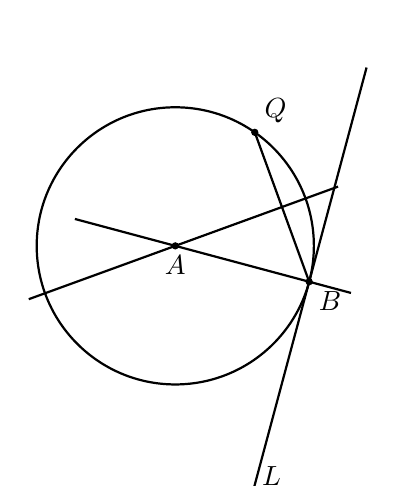
\begin{tikzpicture}[>=latex, scale=1.1]
  \coordinate (A) at (0, 0);
  \draw[thick] (A) circle (1.6);
  \fill (A) circle (1.2pt) node[below] {$A$};
  
  % Tangent point B at angle -15 deg
  \coordinate (B) at (-15:1.6);
  \fill (B) circle (1.2pt) node[below right] {$B$};
  
  % Normal to L through B (line AB extended)
  \draw[thick] (-15:-1.2) -- (-15:2.1);
  
  % Tangent line L perpendicular to AB at B
  \draw[thick] ($(B)!-1.6!90:(A)$) -- ($(B)!1.6!90:(A)$) node[above right] {$L$};
  
  % Point Q on circle at angle 55 deg
  \coordinate (Q) at (55:1.6);
  \fill (Q) circle (1.2pt) node[above right] {$Q$};
  
  % Chord BQ
  \draw[thick] (B) -- (Q);
  
  % Perpendicular bisector of BQ through center A (direction angle 20 deg)
  \draw[thick] (20:-1.8) -- (20:2.0);
\end{tikzpicture}
\end{center}

\begin{prop}[命題 4]
若 $C$ 與 $C'$ 不相交，則由 $C$ 與 $C'$ 所產生的共軸圓系中含有兩個點圓．
\end{prop}

\begin{proof}
因圓系中的一般圓 $C_t$ 的方程式為
\[
C_t:\; x^2+y^2+2\left(\frac{D+tD'}{1+t}\right)x + 2\left(\frac{E+tE'}{1+t}\right)y + \left(\frac{F+tF'}{1+t}\right) = 0
\]
$C_t$ 的半徑為
\begin{align*}
r_t &= \sqrt{\left(\frac{D+tD'}{1+t}\right)^2 + \left(\frac{E+tE'}{1+t}\right)^2 - \frac{F+tF'}{1+t}} \\
&= \frac{1}{|1+t|} \sqrt{(D+tD')^2 + (E+tE')^2 - (1+t)(F+tF')}
\end{align*}
欲證此圓系含有兩個點圓，須證存在兩個相異 $t$ 值使得 $r_t = 0$．令 $r_t = 0$ 即
\[
(D+tD')^2 + (E+tE')^2 - (1+t)(F+tF') = 0
\]
或
\[
({D'}^2+{E'}^2-F')t^2 + 2\left(DD'+EE'-\frac{F+F'}{2}\right)t + (D^2+E^2-F) = 0.
\]
上式有二相異實根的條件為
\[
\left(DD'+EE'-\frac{F+F'}{2}\right)^2 - (D^2+E^2-F)({D'}^2+{E'}^2-F') > 0
\]
此即為 $C$ 與 $C'$ 兩圓不相交的條件（習題 III-6 第 4 題）．
\end{proof}

\subsection*{§ 2\quad 共軛的共軸圓系}
\addcontentsline{toc}{subsection}{§ 2\quad 共軛的共軸圓系}

設 $\{C_t \mid t \in \mathbf{R}\}$ 是由兩個不同心的圓 $C$ 與 $C'$ 所產生的共軸圓系，而 $\{\bar{C}_{t'} \mid t' \in \mathbf{R}\}$ 是由兩個各與 $C$ 與 $C'$ 正交的圓 $\bar{C}$ 與 $\bar{C}'$ 所產生的共軸圓系，我們將證明一圓系中的圓與另一圓系中的圓互相正交．

\begin{proof}
設圓 $C, C'; \bar{C}, \bar{C}'$ 的方程式分別為
\begin{align*}
C:&\; x^2+y^2+2Dx+2Ey+F=0 \\
C':&\; x^2+y^2+2D'x+2E'y+F'=0 \\
\bar{C}:&\; x^2+y^2+2\bar{D}x+2\bar{E}y+\bar{F}=0 \\
\bar{C}':&\; x^2+y^2+2\bar{D}'x+2\bar{E}'y+\bar{F}'=0
\end{align*}
則由 $\bar{C}$ 和 $C$ 及 $C'$ 正交，及 $\bar{C}'$ 和 $C$ 及 $C'$ 正交的條件得
\begin{align}
2D\bar{D} + 2E\bar{E} - (F+\bar{F}) &= 0 \label{eq:b4-a2-c1} \\
2D'\bar{D} + 2E'\bar{E} - (F'+\bar{F}) &= 0 \label{eq:b4-a2-c2} \\
2D\bar{D}' + 2E\bar{E}' - (F+\bar{F}') &= 0 \label{eq:b4-a2-c3} \\
2D'\bar{D}' + 2E'\bar{E}' - (F'+\bar{F}') &= 0 \label{eq:b4-a2-c4}
\end{align}
\eqref{eq:b4-a2-c1} $+ t$ \eqref{eq:b4-a2-c2} $+ t'$ \eqref{eq:b4-a2-c3} $+ tt'$ \eqref{eq:b4-a2-c4} 得
\[
2(D+tD')(\bar{D}+t'\bar{D}') + 2(E+tE')(\bar{E}+t'\bar{E}') - [(F+tF')+(\bar{F}+t'\bar{F}')] = 0.
\]
上式即表示 $C_t$ 與 $\bar{C}_{t'}$ 正交（§ III-6 命題 10）．
\end{proof}

\begin{definition*}
設 $\{C_t \mid t \in \mathbf{R}\}$ 和 $\{\bar{C}_{t'} \mid t' \in \mathbf{R}\}$ 為兩個共軸圓系，若前一圓系中任意一圓 $C_t$ 和後一圓系中任意一圓 $\bar{C}_{t'}$ 均互相正交，則稱此二圓系\textbf{互為共軛的共軸圓系}．
\end{definition*}

\begin{example-non}[例 1]
設 $L$ 與 $L'$ 為二正交於 $O$ 點的直線，則由命題 $3'$ 知：

所有和 $L$ 相切於 $O$ 點的圓做成一共軸圓系 $\{C_t \mid t \in \mathbf{R}\}$，

所有和 $L'$ 相切於 $O$ 點的圓做成一共軸圓系 $\{\bar{C}_{t'} \mid t' \in \mathbf{R}\}$，

顯然此二圓系是互為共軛的共軸圓系． \hfill $\#$
\end{example-non}

\begin{center}
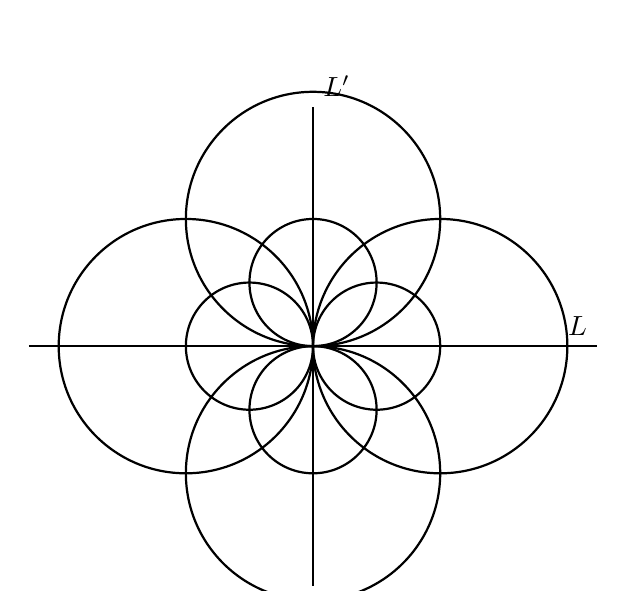
\begin{tikzpicture}[>=latex, scale=0.95]
  \draw[thick] (-3.8,0) -- (3.8,0) node[above left] {$L$};
  \draw[thick] (0,-3.2) -- (0,3.2) node[above right] {$L'$};
  
  % 2 circles in each direction tangent at origin O (8 circles total)
  \foreach \r in {0.85, 1.7} {
    \draw[thick] (0, \r) circle (\r);
    \draw[thick] (0, -\r) circle (\r);
    \draw[thick] (\r, 0) circle (\r);
    \draw[thick] (-\r, 0) circle (\r);
  }
\end{tikzpicture}
\end{center}

\newpage
\begin{example-non}[例 2]
設 $A_1(a_1, b_1)$ 及 $A_2(a_2, b_2)$ 是平面上兩定點．令直線 $A_1 A_2$ 為 $L$，線段 $\overline{A_1 A_2}$ 的垂直平分線為 $L'$．則由命題 3 知：

所有過 $A_1$ 及 $A_2$ 的圓做成一個共軸圓系 $\{C_t \mid t \in \mathbf{R}\}$．

又由兩點圓 $\bar{C}_1 = \{A_1\}$ 及 $\bar{C}_2 = \{A_2\}$ 所產生的共軸圓系為
\[
\{\bar{C}_{t'} \mid \bar{C}_{t'}: [(x-a_1)^2+(y-b_1)^2] + t'[(x-a_2)^2+(y-b_2)^2] = 0, \; t' \in \mathbf{R}\}
\]
因為點圓 $\bar{C}_1$ 及 $\bar{C}_2$ 與 $C_t$ 正交，故知上二圓系互為共軛的共軸圓系． \hfill $\#$
\end{example-non}

\begin{center}
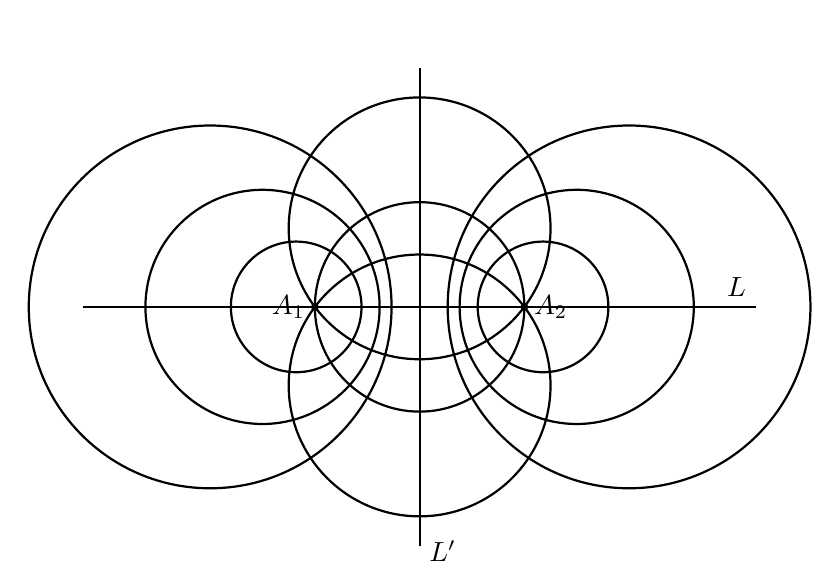
\begin{tikzpicture}[>=latex, scale=0.95]
  \coordinate (A1) at (-1.4, 0);
  \coordinate (A2) at (1.4, 0);
  
  \draw[thick] (-4.5,0) -- (4.5,0) node[above left] {$L$};
  \draw[thick] (0,-3.2) -- (0,3.2);
  \node[below right] at (0,-3.0) {$L'$};
  
  \fill (A1) circle (1.5pt) node[left] {$A_1$};
  \fill (A2) circle (1.5pt) node[right] {$A_2$};
  
  % 3 Circles passing through A1 and A2 (centers on L')
  \draw[thick] (0, 0) circle (1.4);
  \draw[thick] (0, 1.05) circle ({sqrt(1.05*1.05 + 1.4*1.4)});
  \draw[thick] (0, -1.05) circle ({sqrt(1.05*1.05 + 1.4*1.4)});
  
  % 6 Orthogonal Apollonian circles (limiting points A1, A2, centers on L)
  % r = sqrt(k^2 - 1.4^2)
  \foreach \k in {1.65, 2.1, 2.8} {
    \pgfmathsetmacro{\rad}{sqrt(\k*\k - 1.4*1.4)}
    \draw[thick] (\k, 0) circle (\rad);
    \draw[thick] (-\k, 0) circle (\rad);
  }
\end{tikzpicture}
\end{center}


\end{document}
